\chapter{Отчет ведущего научного сотрудника ОМИ ДНЦ РАН 0.5 ст. д.ф.-м.н., проф. Магомедова А.М. за 2022 г.}


\section*{Аннотация}

Направления работы в 2022 году:

\begin{enumerate}
    \item Прикладное программирование. 
    \item Проблемы перечислительной комбинаторики.
    \item Разработка методического, алгоритмического и программного обеспечения.
\end{enumerate}


\section{Прикладное программирование}

Разработаны или существенно улучшены более двадцати программ прикладного программирования; издана монография и подготовлен черновой вариант  учебного пособия по системе компьютерной математики <<Mathematica>>.


\subsection{Построение алгоритмов. Издание монографии}

Подготовлена и издана монография \cite{akm-bib-m1}, все 20 разделов которой посвящены нестандартным проблемам прикладного программирования (первый рецензент -- Шарапудинов Т.И.).   
Основное внимание уделено разработке алгоритмов и обсуждению подходов к решению, не ограничиваясь при решении конкретной задачи одним-единственным алгоритмом; для ряда задач предложены два-три различных алгоритма, воплощенные в одной программе для удобства сравнения по быстродействию; характерной особенностью является многоязычие --- в некоторых программах используется взаимодействие средств двух языков высокого уровня; к некоторым задачам предложены по две программы, написанные на разных языках.
Основное внимание уделено разработке алгоритмов.


\subsection{Разработка программного обеспечения} 

Приоритетным направлением явилась разработка программного обеспечения, призванного: а) осуществлять поддержку теоретических исследований по дискретной математике (\cite{akm-bib-m9, akm-bib-m10, akm-bib-m14, akm-bib-m15}); б) решить нестандартные задачи прикладного характера.


\section{Проблемы перечислительной комбинаторики}

Продолжены исследования по вычислительным аспектам димерных чисел. Найдено простое доказательство существования прямого рекуррентного соотношения для последовательности димерных чисел прямоугольной полосы при произвольно фиксированной ширине полосы. Усовершенствован алгоритм проверки существования интервальной раскраски у двудольного графа заданного порядка (известная NP-полная задача).


\subsection{Димерные числа}

В 2022 г. одним из основных направлений нир явилось продолжение исследования проблемы димерных чисел, другими словами, -- задачи вычисления числа $T(m,n)$ совершенных паросочетаний в решёточном графе заданных размеров $m\times n$. Известно, что $T(m,n)$ равно числу всевозможных разбиений прямоугольной полосы $m\times n$ на плитки $1\times 2$. При фиксированной ширине $m$ принято обозначать $T(m,n)$ через $a_n$. Все известные из литературы прямые рекуррентные соотношения для $a_n$ (т.е. представление $a_n$ в виде линейной комбинации $a_0, a_1,..., a_{n-1}$ с целыми постоянными коэффициентами) получены исходя из того, что факт существования таких прямых рекуррентных соотношений априори известно.

В 2022 г. найдено непосредственное и краткое доказательство данного факта. Это основной результат за 2022 г.

Отметим второй результат в данном направлении. Все полученные ранее рекуррентные соотношения для 
$a_n$ (при фиксированном $m$) выводились с использованием двухступенчатой схемы: сначала формировалась система взаимно рекуррентных формула (с.в.р.ф.) для $a_n, b_n, c_n, \dots$ (где $b_n, c_n, ...$  --- димерные числа для фигур, полученных из исходного прямоугольника удалением некоторых клеток верхней строки), затем из с.в.р.ф. методом исключения находили $a_n$ (см., например, \cite{akm-bib-m3}). В текущем году удалось получить рекуррентное соотношение для $a_n$ без использования двухступенчатой схемы (однако распространить результат на $m>4$ не удалось).

\underline {Прикладное значение}. Изучение ряда свойств химического соединения можно эффективно проводить, исследуя топологическую модель молекулы, т. е. представляя молекулу в виде неориентированного графа, в котором вершины соответствуют атомам, а ребра — химическим связям; 
некоторые классы химических соединений успешно синтезируются только тогда, когда графы соединений имеют совершенное паросочетание; 
компоненты некоторых семейств соединений тем стабильнее, чем больше совершенных паросочетаний в их графах.
	
Задача возникает и при исследовании адсорбции двухатомных молекул на поверхности: требуется найти число способов объединения атомов в двухатомные молекулы (димеры), так чтобы при этом покрывалась дважды периодическая решётка с шагом, равным длине димера, причём каждый димер покрывал бы две смежные точки решётки и не оставалось бы ни одной непокрытой точки.


\subsection{Интервальная раскраска двудольных графов}

Разработанный ранее для проверки существования у двудольного графа  интервальной раскраски алгоритм усилен фрагментом, названным 
<<Методом $c$-увеличивающего пути>>. Приведем его краткое описание, где через $LC[v_k]$ обозначен интервал цветов, представленных в вершине $v_k$, через $C[i_k]$ -- цвет ребра с номером $i_k$.
 
Вершинно-непересекающийся путь из чередующихся ребер (не окрашено -- окрашено в цвет $c$, не окрашено --- окрашено в цвет $c$ -…-  не окрашено): 
$$v_1-v_2-v_3-\dots-v_d$$  
будем называть <<c-увеличивающим>>, если цвет $с$ является граничным для интервалов $LC[v_1]$ и $LC[v_d] $ и входит в интервалы цветов всех внутренних вершин пути: $v_2,v_3, \dots, v_{d-1}$. 
Номера последовательных ребер c-увеличивающего пути обозначим $i_1, i_2, \dots, i_{d-1}$ и выполним действия, увеличивающие число окрашенных ребер пути с сохранением цветов всех ребер, не принадлежащих данному пути:

окрасим ребро $(v_1,v_2)$ в цвет $c$ и удалим цвет ребра $(v_2,v_3)$, окрасим ребро $(v_3,v_4)$ в цвет $c$ и т.д.:

$C[i_1 ]=c, LC[v_1].Add(c);$

$C[i_2]=-1; C[i_3]=c; C[i_4 ]=-1; C[i_5 ]=c; \dots ,C[i_{d-2}]=-1;$

$C[i_{d-1}]=c; LC[d].Add(c)$.

Усиленный описанным методом алгоритм (в реализации \cite{akm-bib-m14, akm-bib-m15}) легко справился с задачей нахождения интервальной раскраски у графа на рис.~\ref{akm-fig-1}. На рисунке вторые метки ребер --- номера цветов.
\begin{figure}[h]
    \begin{center}
        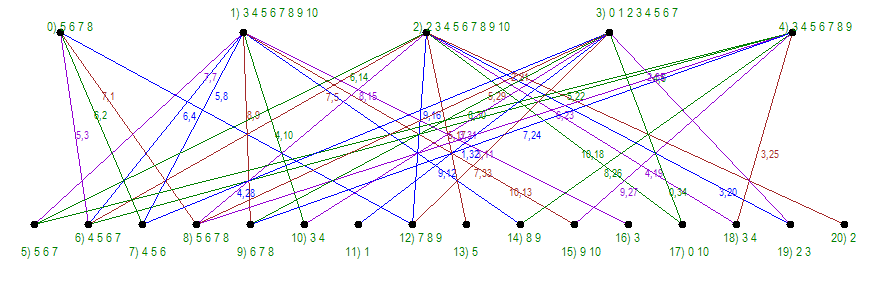
\includegraphics[width=1.0\textwidth]{akm/int.png}
    \end{center}
    \caption{Интервальная раскраска двудольного графа порядка 21, найденная программой. Первая метка ребра -- его номер, вторая метка -- номер цвета ребра. Около каждой вершины 0), 1), ..., 20)  указан список цветов, представленных в данной вершине.}
    \label{akm-fig-1}
\end{figure}

\underline{Прикладное значение.} Интервальная раскраска двудольного графа $(X,Y,E)$ является графической интерпретацией беспростойного расписания мультипроцессорной системы,  где $X$ -- процессоры, $Y$ -- задания, $(x,y) \in E$ если и только если процессору $x$ предписано обработать задание $y$. 


\subsection{Симплициальные комплексы заданного типа} 

Ранее в соавторстве с Лавренченко C. А.  была опубликована статья, где вводится новый перечислительный многочлен для абстрактных комплексов заданного типа, например, деревьев с фиксированным числом вершин или триангуляции тора с фиксированным графом. 
Дальнейшее развитие идей статьи (в направлении исследования свойств вычислительного многочлена) опубликовано в качестве главы 8 в монографии \cite{akm-bib-m3}. 


\section{Разработка методического, алгоритмического и программного обеспечения}
  
Разработаны (в некоторых случаях значительно доработаны частично разработанные ранее программы) и зарегистрированы в гос.реестре программы для ЭВМ, предназначенные для решения перечислительных проблем дискретной математики, компьютерной графики и создания демонстрационного материала по дисциплинам компьютерных наук.


\subsection{Поиск с масштабируемым контекстом в произведениях на языке народа Дагестана (на примере аварского языка)}
\begin{figure}[h]
    \begin{center}
        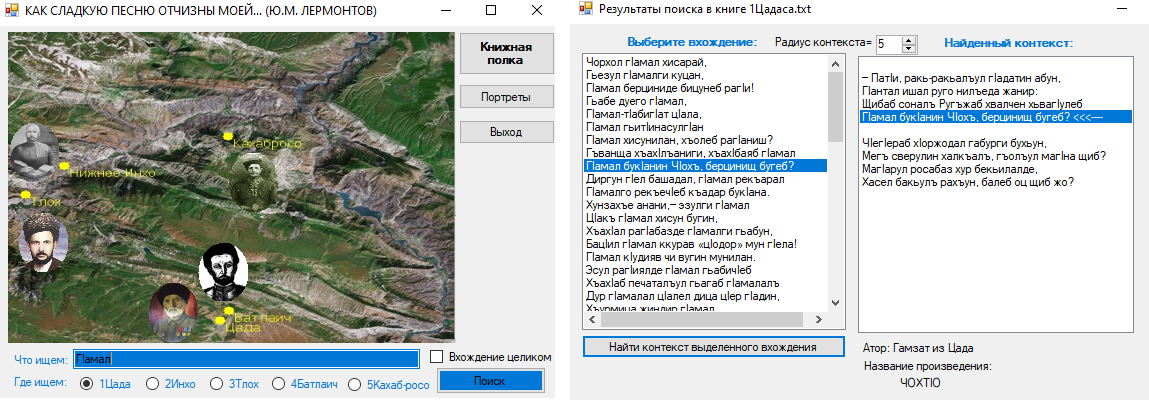
\includegraphics[width=1.0\textwidth]{akm/lit.png}
    \end{center}
    \caption{Поиск с масштабируемым контекстом.}
\end{figure}

Функциональность: а) выбор и отображение литературного произведения для гипертекстового просмотра в окне из трех фреймов: в верхнем - список авторов, в левом фрейме - список ссылок - названий произведений выбранного автора, в правом фрейме выводится текст соответствующего произведения;
б) устойчивый к нечеткости набора поиск наименования произведения и фамилии автора по заданному фрагменту текста.


\subsection{Визуальное восприятие дискретных серий сигналов}

Разработана C\#-программа с существенным повышением надежности разработанного ранее программного обеспечения (на Delphi) для оцифровки серий дискретных звуковых сигналов.

Перспективы: а) анализ программной оцифровки изображения в окне редактора звуков; 
б) разработка программы для отображения на экране буквы выполнением 2-серийной дискретной последовательности движений глазами; в) усиление функциональности программы до вывода на экран текста в результате выполнения серий дискретных движений глазами. 

\underline{Ожидаемое применение.}
Для общения с обездвиженным пациентом;  в ежедневном быту лиц со слабым слухом.
\begin{figure}[h]
    \begin{center}
        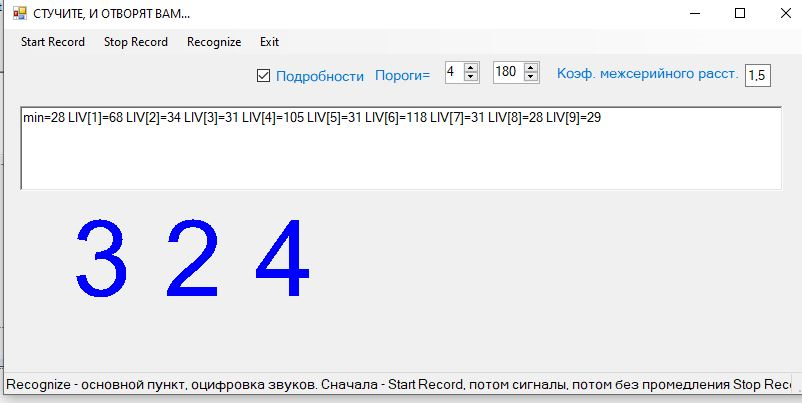
\includegraphics[width=1.0\textwidth]{akm/audio.png}
    \end{center}
    \caption*{Визуальное восприятие дискретных серий сигналов.}
\end{figure}


\subsection{Создание карты Республики Дагестан}

Цели проекта: - разработка 2-мерной муниципальной карты РД с масштабированием и детализацией актуальной местности; поиском населенных пунктов; границ районов; маршрутов; подробной текстовой и графической информацией о выбранном районе или населенном пункте; - частичное решение задачи разработки 3-мерной физической карты РД.
\begin{figure}[h]
    \begin{center}
        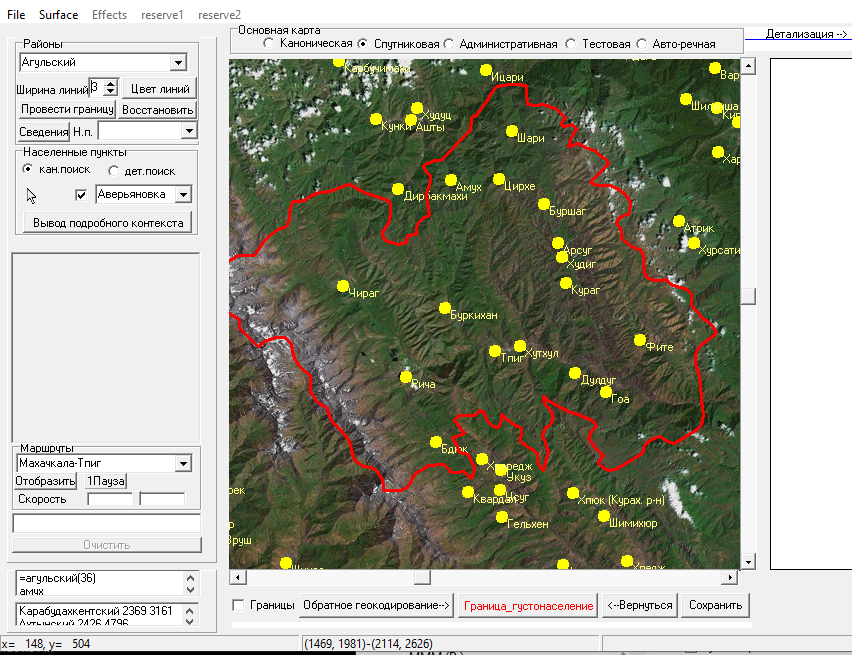
\includegraphics[width=1.0\textwidth]{akm/RDmap.png}
    \end{center}
    \caption*{Создание карты Республики Дагестан.}
\end{figure}
\underline{Примеры пунктов, завершенных к настоящему времени}: <<бесшовное>> склеивание электронной карты РД из отсканированных фрагментов,
просмотр карты значительных размеров путем прорисовки в окне просмотра лишь востребованного в текущий момент фрагмента малых размеров $(512\times 512)$; способы указания в интерактивном режиме выбранного населенного пункта (н.п.): из локального списка названий н.п. текущего района и/или из глобального списка, вводом названия в редактируемое поле или визуальным указанием на карте. 


\subsection{Реставрация рукописи}

Программа предназначена для распознавания точек на изображении рукописи: а) фона и б) текста. Цель и задачи программы: замена зашумленного фона рукописного текста однородным или выбранным пользователем фоном, изменение толщины и цвета текста.
Программу рекомендуется использовать для реставрации старых рукописей. 

\begin{figure}[h]
    \begin{center}
        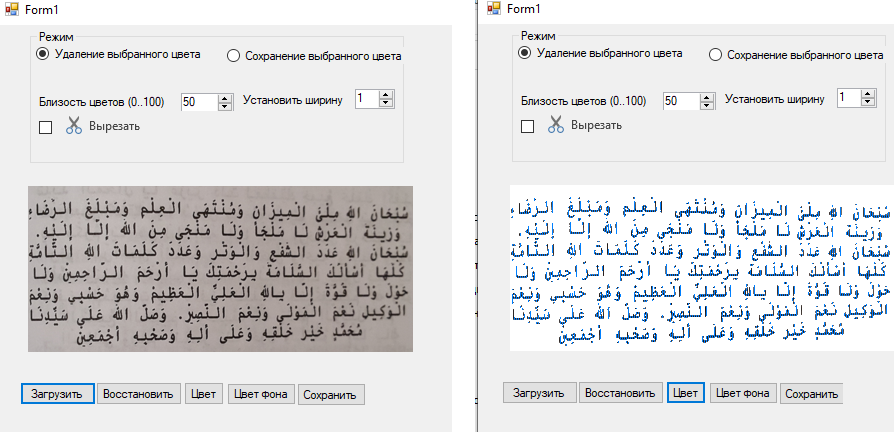
\includegraphics[width=1.0\textwidth]{akm/arab.png}
    \end{center}
    \caption*{Реставрация рукописи. Слева -- исходный рисунок, справа -- результат работы программы.}
\end{figure}


\section{Заключение}

За 2022 г. автором издана монография, опубликованы  в изданиях из списка ВАК  четыре статьи, еще две публикации в сборнике трудов Всероссийской конференции, получены восемь свидетельств о государственной регистрации в Реестре программ для ЭВМ, а также опубликована глава в монографии зарубежных авторов. В 13 из 16 публикаций (а также приравненных к ним) указано, что они выполнены благодаря поддержке ОМИ ДФИЦ РАН.
